
%% PLANUNG %% 

\chapter{Conception and Design}
This section deals with the conception of the graphical user interface and the implementation options of the application.
\section{Graphical User Interface}
First it needs to be determined whether the graphical user interface plays a vital role in applications. For this purpose, a question on this topic was also included in the first survey. The answers to this question revealed that the graphical interface of an application plays an important role in terms of the trustworthiness of the application. Figure 6.1 shows the results of the survey question.
\begin{figure}[H]
	\centering
	\includegraphics[scale=0.4]{appUiImportant.png}
	\caption[Survey Question]{Survey Question - Trustworthiness of the Application based on the UI}
\end{figure}
\noindent
Respondents to the survey were also allowed to choose between three different UIs. The graphical interface should be adapted to the choice made by the people interviewed.
\subsection{Conceptual Design of the Graphical User Interface}
The UI can be designed based on the requirements analysis of the application and the information obtained from it. As already defined, the application should be designed to be as intuitive and easy to use as possible. The implementation of the design of the user interface for the Android version is based on suggestions from the material.io website \cite{.materialio}, an open-source design system developed by Google. The integration of the design components into the Flutter application is simplified thanks to the pre-installed material.dart package. This package is based on the source mentioned and currently supports version 2 of material.io. Support for the current version 3 of Material Design is still being worked on.
\noindent
One goal of this application is to be designed to be intuitive. In his book "UI is COMMUNICATION", Everett N. McKay described an intuitive UI as follows \cite{.mckay}: 
\begin{quote}
	\textit{"A UI is intuitive when target users understand its behavior and effect without use of reason, memorization, experimentation, assistance, or training."} - Everett N McKay \cite[p. 22]{.mckay}
\end{quote}
In order to meet this definition, goals that the user interface should meet could be set before the graphic user interface is designed.\\
\noindent
The user should be able to recognize immediately that a component of the screen is a widget that he can operate. The system must then show the user that his action has triggered something. This can be done, for example, through feedback in the form of a loading circle if required data still needs to be loaded or in the form of a new screen, pop-up, or similar design components. \cite{.mckay} Another step that can be taken to make the application more intuitive is the correct (short) labeling of the respective components. For example, a corresponding text, or even better imagery \cite[p. 172]{.essui}, should be stored on a confirmation button. In addition, it should be ensured that surface components do not change their positions. This establish that users can rely on their previous interactions and thus learn how to use the application. Minimalism is becoming a trend not only in the real world but also in the digital world. This can also be recognized by looking at large companies' graphical development of various icons and web interfaces.
\begin{figure}[H]
	\centering
	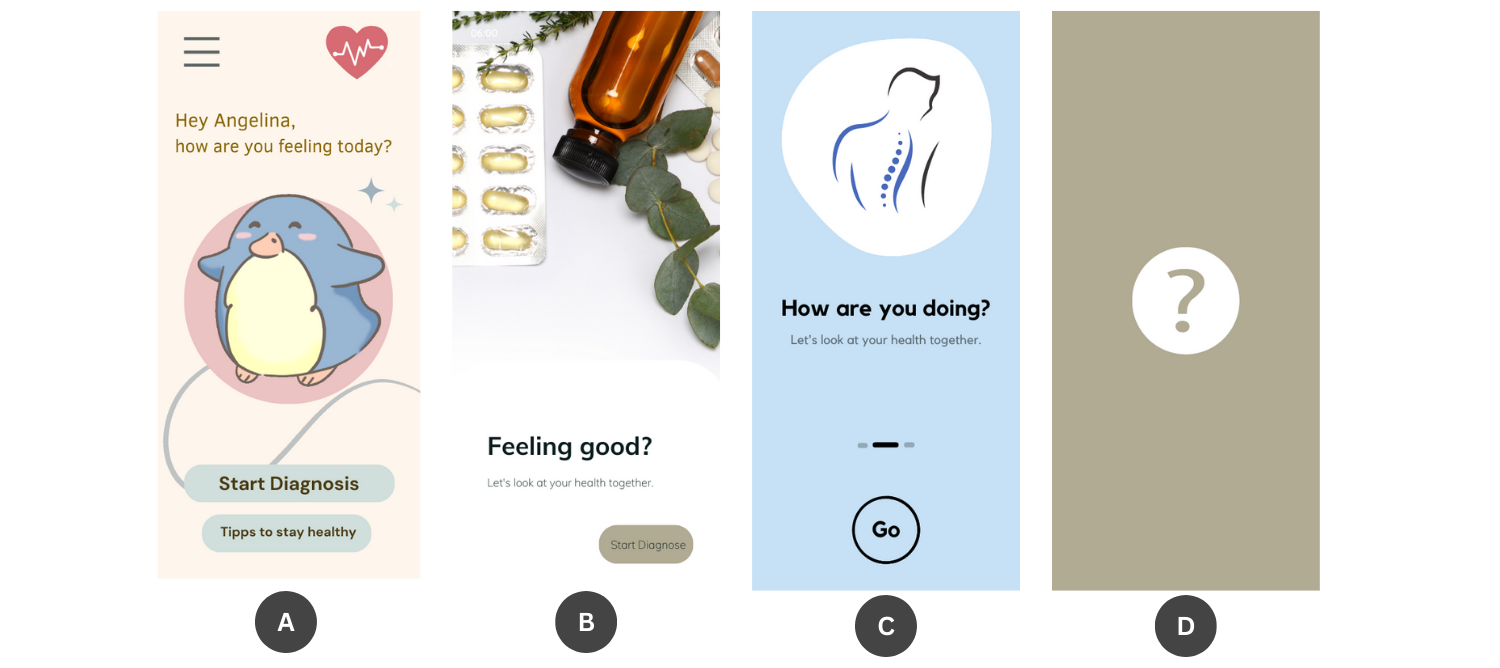
\includegraphics[scale=0.4]{whichUIPics.png}
	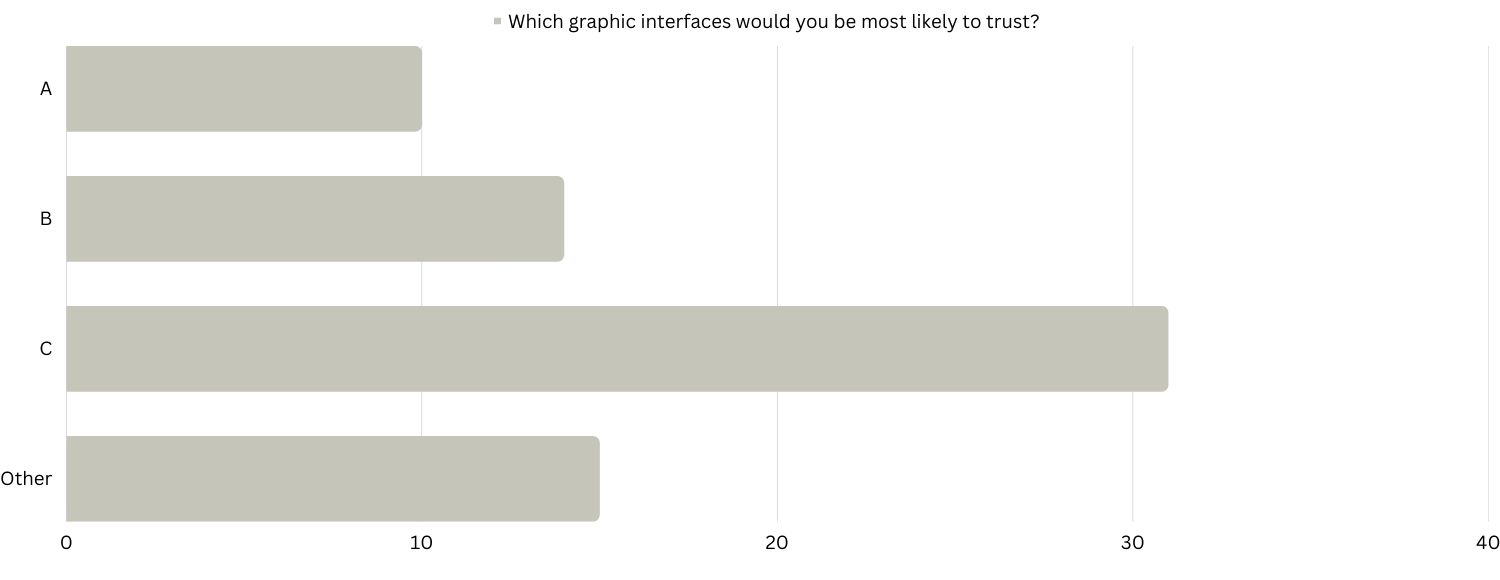
\includegraphics[scale=0.4]{whichUI.png}
	\caption[Survey Question]{Survey Question - Which UI would respondents like the most}
\end{figure}
\noindent
Designing the application as minimalistic as possible has the advantage that the graphical interface is not overloaded; thus, the user is not overwhelmed by different widgets. This may make it easier for the user to interpret specific elements better. Another factor that plays a role in user-friendliness is using familiar design patterns. This ensures that users are already familiar with handling the app elements and that everything is clear regarding the use. 

\subsection{Description of the Views and Thoughts on the Implementation in Flutter}
This section presents the individual views that are made available to users. In addition, first thoughts on possible ways of implementation for those views, working with Flutter, are considered.
\subsubsection{\textbf{Home Screen}}
The home screen is the first view a user will encounter when installing or opening the application. He should be allowed to switch between the different views necessary for his use: diagnosis creation, diagnosis overview, and advice view. In addition, every user should be able to access the login screen for doctors since they can verify themselves there. The navigation to create a diagnosis is implemented as a button and labeled with a corresponding, clearly formulated text. To get to all other screens, a list view of all options is offered, in which various clickable fields trigger navigation to the corresponding screen when clicked. In Flutter, this view can be achieved through several different components. Essential widgets can be used as children in a column. In order to implement the clickable forwarding elements to other views, one should use a ListView, storing children of the widget GestureDetector, which allows any widget to be clickable. The children can be stored in an external modifiable list, simplifying the integration of new categories later in time.

\subsubsection{\textbf{View for the Diagnostic Process}}
The screen to start a diagnosis should be designed as simple as possible. Users can address which body part they are experiencing their symptoms. Based on their selection, the application shows all symptoms associated with the body part, which can be selected and afterward specified by the user. The widget \textit{Stepper} is a possible implementation option. It allows the developer to implement a type of step-by-step tool quickly. For this purpose, only all steps for generating a diagnosis are created and filled with the appropriate data. The complete code for an abbreviated Stepper widget can be found in Appendix I.

\subsubsection{\textbf{Login Screen (Doctor)}}
The login screen is displayed to the user immediately after clicking on the navigation tool labeled "Doctor Panel". There he will be offered the option to log in or register. This is achieved by adding editable text fields for the needed user input: email, password, and confirmation password. If the user has already created a user account in a previous session, has verified himself as a medical professional, and has then been logged in, he will be forwarded to the actual doctor panel without needing to log in. An exception is given if he has previously logged out. With the help of the flutter\_login package, a developer can quickly implement the login process in Dart. There are also options to customize the appearance of the login form.

\subsubsection{\textbf{Screen with all Body Parts, Diseases, Advice, and Symptoms (Doctor Panel)}}
The doctor panel should contain all the necessary data related to the records stored in the database. Here, doctors can switch between the different collections. A suitable implementation method for this would be the BottomNavigationBar. It contains various navigation elements that change their data view when clicking on them. The data views show a list of stored data in the associated Firestore collection. When the user clicks on such an element, the system redirects to the edit view for the associated record. In order to be able to store new data quickly, a FloatingActionButton can also be integrated, which opens a small menu by clicking on it, where all the data add options for the doctor are listed. Clicking on a listing item then opens the associated add view.

\subsubsection{\textbf{View for adding and editing Data (Doctor)}}
In order to make the views as intuitive as possible, it is advisable to make the graphical interface as uncluttered as possible. Because of this, only text fields are included for the data records where possible. For selecting related data for a data set (e.g., symptoms for an illness), a button is placed on the view, which, when clicked, generates and displays a dialogue with the content of all symptoms in the database. Ideally, this dialog should also contain a search bar so that the user is not forced to scroll through many data records. The edit view and the view to add new records consist of a form widget. There, it is possible to add text fields as children, which users can modify. The distinction here is only between the initial value of the text fields. While the data stored in the database for the associated data record is displayed in the edit view, only an empty text field with a hint regarding the data field is specified when a new data tuple is created.

\subsubsection{\textbf{View with all Saved Diagnoses}}
A vertical list of all diagnoses represents the diagnoses view. A ListView is used here. This ListView contains all diagnostic data that the user has previously saved on his device. Clicking on a diagnosis element in the list opens a detailed view of this diagnosis. It shows the date on which the diagnosis was made, which symptoms the user specified, and which illnesses resulted from calculating the probability of diseases. This is represented in the form of a bar chart. At the end of the diagnosis, the diseases are again listed in list form, with their description and treatment recommendations.

\subsubsection{\textbf{View with all advice stored in the database (User) }}
The advice screen can be designed similarly to the diagnosis screen. Here, the data from Firestore is displayed in the form of a vertical list. A click opens the detailed description of the advice. This detailed view consists of text fields containing the document fields' data.

\subsection{Mock-ups and Survey regarding the Trustworthiness of Mock-up Designs}
With the description of the screens and the first development approaches, mock-ups can already be created with the help of Canva. These can be found in Appendix H. As part of a second survey the participants were asked if the general graphic design looked trustworthy to them, and also if the navigation trough the app was intuitive. The result of this survey showed, that the interface is already widely accepted regarding the mentioned aspects. The detailed results can be found in Appendix G. One interviewee noted that the application should be designed more modernly in some places and should also have simplified data provision. Other points were also specified. These can also be found in Appendix G.

%v
\chapter{Implementation}
Based on the specifications from the previous chapter, it is now possible to look at implementation ideas. This chapter describes the technologies used for the development of this application. The project structure is also examined in more detail.
\section{Project Structure}
When developing a software system in the client-server, it is recommended to make sure that the project and class structures are divided into three (four, if the data layer is counted too - here the data layer is the Firestore Database) different layers \cite[p. 175]{.3layer}.
\begin{itemize}
	\item \textbf{Data Access Layer}
	\newline
	The data access layer retrieves the (raw) data from the database. For this purpose, a class named DatabaseService is generated as part of the Flutter application, which can be instantiated.
	\scriptsize
	\begin{lstlisting}[caption=Stepper for Body Part Selection]
		class DatabaseService {
			/* CREATE AN INSTANCE OF THE DATABASE */
			DatabaseService._();
			static DatabaseService _instance = DatabaseService._();
			static DatabaseService get instance => _instance;
		}
	\end{lstlisting}
	\normalsize
	Using DatabaseService.instance.\_methodName, each method of the service can now be called globally from anywhere in the project.
	\item \textbf{Business Logic Layer}
	\newline
	With the help of the business layer, the data that is now received from the database service can be converted into models with which the system can work accordingly. For this purpose, a ConvertService can be created similar to Listing 7.1, which can be instantiated similarly. This now queries the data using the DatabaseService.instance and converts the data, which is supplied by the Firestore API in the form of DocumentSnapshots, Streams, or QuerySnapshots. The data models for this are presented in the Data Models section.
	\item \textbf{Presentation Layer}
	\newline
	This layer takes care of mapping the data to the graphical interface. To do this, it queries the model data of the ConvertService and creates the widgets that are to be displayed accordingly.
\end{itemize}
In project development, it is increasingly interesting how applications receive their data. As part of this work, this will happen through API queries to the Firestore database. The whole procedure is also known as the client-server model. An example of the communication process, together with the services that just got described, is shown in Figure 7.1. 
\begin{figure}[H]
	\centering
	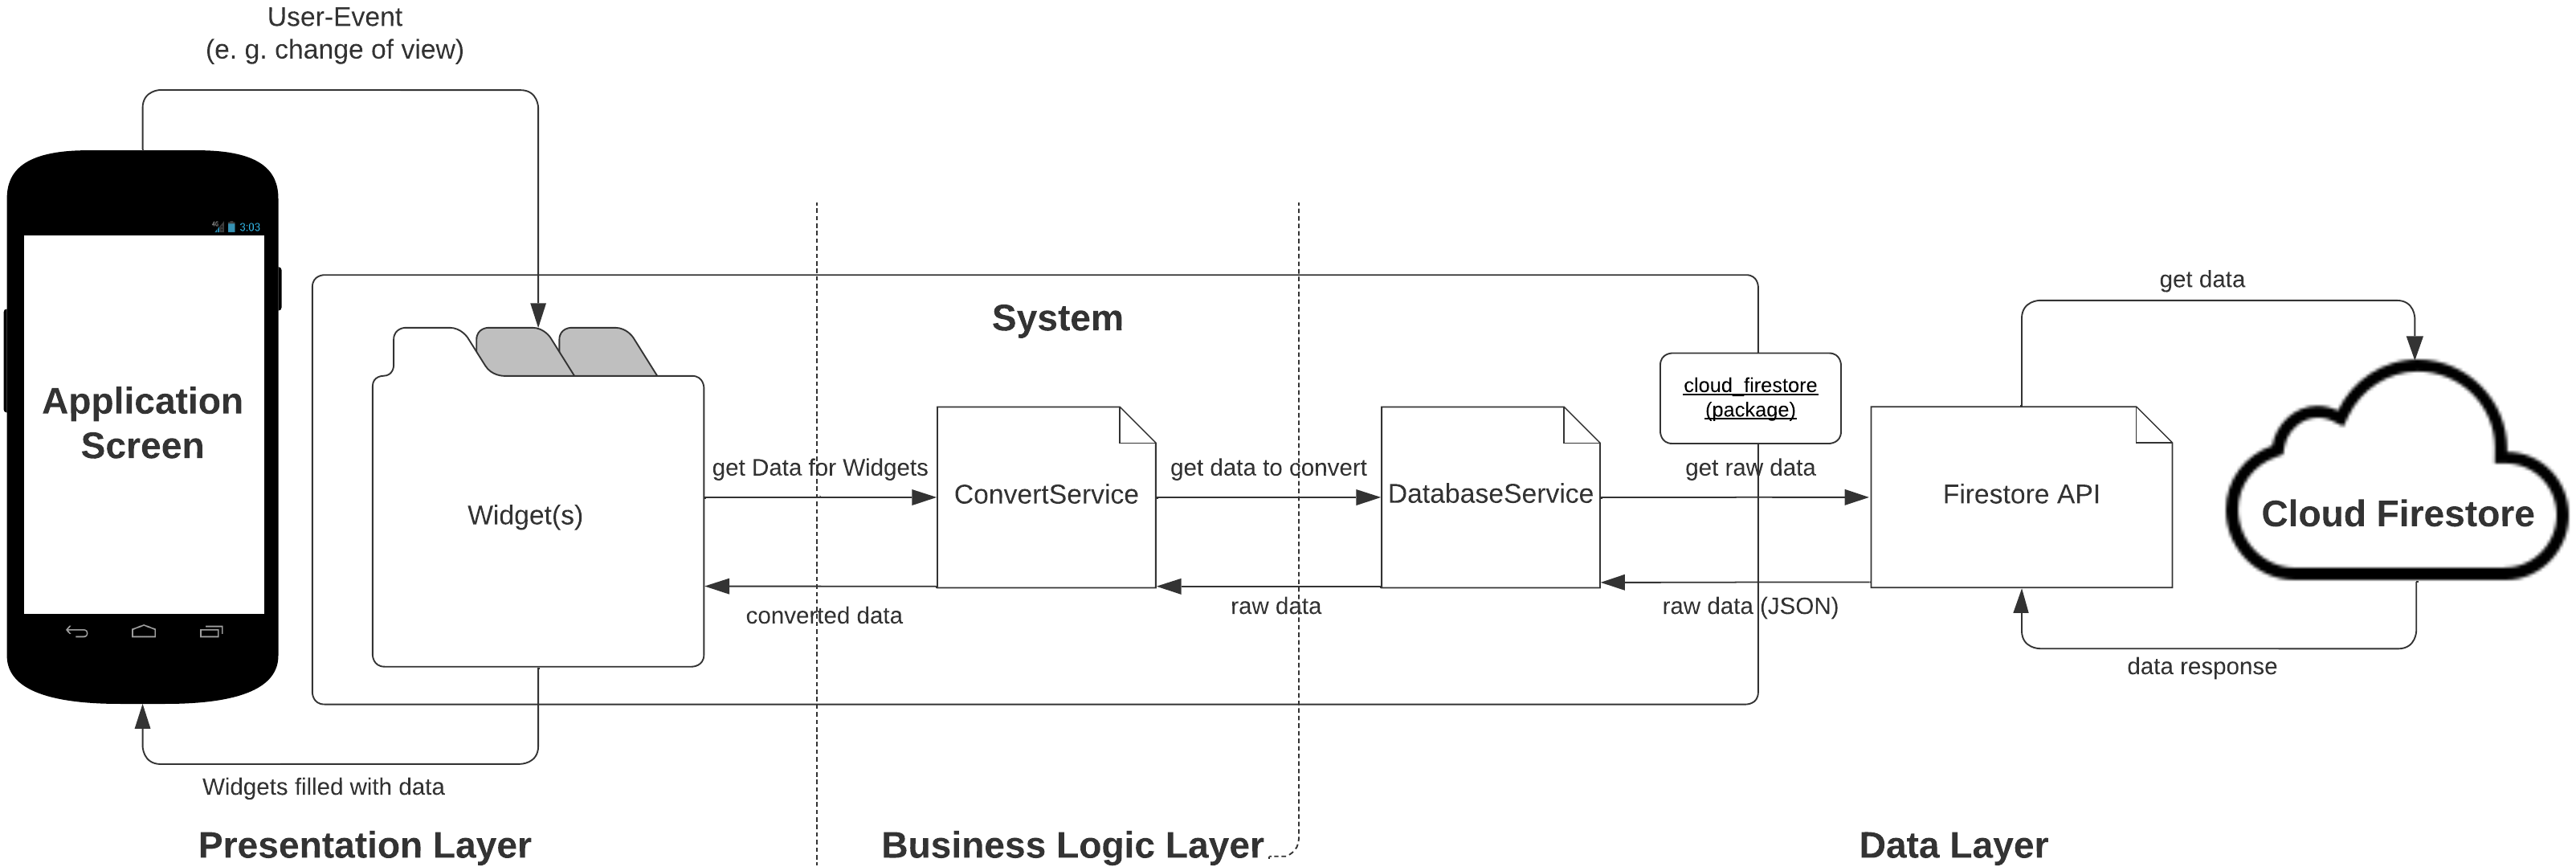
\includegraphics[scale=0.2]{api_flow.png}
	\caption[Client-Server Request Flow]{Client-Server Request Flow}
\end{figure}
\noindent
\subsection{Routing in the Application}
Another step that can be taken to keep the project structure as clean as possible is to lay out the navigation in an extra class. In this work, a class that is named AppNavigator is created for this purpose. This navigator can then be called globally using a defined method AppNavigator.push(Route pRoute). The route parameter is an element of an enumeration which refers to different views of the application. All AppNavigator code can be found in Appendix J.3.
\section{Data Models}
The data model into which the ConvertService converts the raw data of the DataService is based on the document structure stored in the database. When scraping the data of the JSON responses, the data is converted as follows: String$\,\to\,$String, Array$\,\to\,$List, Map<key, value>$\,\to\,$ map < String, dynamic>, Number$\,\to\,$num. Listing 7.2 shows the resulting model for symptoms.
\scriptsize
\begin{lstlisting}[caption=Model for Symptoms]
	class Symptom {
		final String? id;
		String name;
		List<String> symptoms;
		
		Symptom({this.id, required this.name, required this.symptoms});
		
		Map<String, dynamic> toMap() {
			return {
				'name': name,
				'proposed_symptoms': symptoms
				};}
		
		Symptom.fromDocumentSnapshot(DocumentSnapshot<Map<String, dynamic>> doc)
		: id = doc.id,
		name = doc.data()!["name"],
		symptoms = doc.data()!["proposed_symptoms"];	
	}
\end{lstlisting}
\normalsize


\section{Algorithms for the Attribution of Symptoms to potential Diseases}
\subsection{List Matching}
The first methodology to be considered is based on purely theoretical aspects. By specifying the symptoms given by the patient, the application compiles a list of them. When adding the diseases to the database, a list of symptoms was also generated in each disease document. An intuitive idea would be to compare these two lists with each other according to a matching algorithm, which calculates the percentage of word matching in the lists. The so-called word matching is described in source \cite{.wordmatching}. However, it should be noted that no medical data is included in the calculation. Accordingly, the probability of the correctness of the diagnosis decreases. In this sense, another, more exact method is to be considered.

\subsection{Machine Learning: Bayes Theorem and Bayesian Networks}
The so-called Bayes theorem is the foundation of the machine learning technique known as naive Bayes \cite[p. 403]{.bayes1}. According to the Bayes theorem, a principle of probability theory, one may determine the likelihood of an event (such as the existence of a disease) based on the likelihood of occurrences that are connected to it (e.g., certain symptoms) \cite[p. 403 ff.]{.bayes1} \cite{.bayes2}. The Bayes theorem is applied in the case of Naive Bayes to forecast classification issues. The model's components are thought to be completely independent of one another \cite{.naivebayes}.
\newline \\
On the other hand, Bayes networks are a particular probabilistic graph type that employs the Bayes theorem to determine the likelihood of occurrences that depend on numerous independent variables \cite{.bayesnet}. In Bayes networks, the edges between variables represent the relationships between them, with the edges' probabilities describing the link's strength. Similar to Naive Bayes, Bayes networks can be used to forecast classification problems, but they can also be used to simulate more intricate relationships between variables  \cite{.bayesnet}. Generally speaking, the Bayes theorem-based methodologies of Naive Bayes and Bayes Networks are used to forecast occurrences. The fundamental distinction is that although Bayes networks represent and model the relationships between variables, Naive Bayes implies that all features are independent. 
\newline \\
To create a Bayesian network for disease calculation, it is first necessary to identify the variables that should be included in the model. These variables will include the various symptoms that are associated with different diseases, as well as the diseases themselves. Once they are identified a graphical representation of the relationships between them can be created by drawing a directed acyclic graph (DAG) \cite{.bayesnet} \cite{.bayesnet2}. In this DAG, the nodes represent the variables, and the edges represent the relationships between the variables. For example, a node for a particular symptom, such as a fever, and another node for a particular disease, such as the flu. Then an edge between the nodes can be created to represent that the presence of a fever is often associated with the flu. It is also possible to assign probabilities to the edges in a Bayesian network to represent the strength of the relationship between the variables. For example, if a fever is a strong indicator of the flu, it might be wise to assign a high probability to the edge between the fever and flu nodes. On the other hand, if it is known that a fever is only a weak indicator of the flu, one might assign a lower probability to the edge.
\newline \\
Once the Bayesian network is created, and probabilities are assigned to the edges, one can use it to make predictions about the likelihood of an individual having a particular disease based on the presence or absence of specific symptoms. For example, if one has a Bayesian network that includes nodes for the symptoms of fever, cough, and sore throat, as well as nodes for the diseases of the flu and the common cold, which is information that the patient entered: In that case, one can use the probabilities assigned to the network's edges to calculate the likelihood that the individual has the flu or the common cold.
\newline \\
In summary, Bayesian networks are a powerful tool for calculating the likelihood of an individual having a particular disease based on the presence or absence of specific symptoms.

\subsection{Algorithmic Solution}
Lastly, the symptom classification described in the conference paper "Towards a ranking of likely diseases in terms of precision and recall" \cite{.algo} is examined. Although the paper was published in 2012. It addresses problems still present today with certain disease classification methods and a solution developed with medical experts on how these methods can be cleanly replaced. The information which can be taken from the paper still offers a reasonable basis for an algorithmic solution to disease determination. 
\newline \\
The paper addresses, among other things, problems that bayesian networks bring with them: the pure information regarding the probabilities of certain diseases is not widespread and accessible or even available \cite{.algo}. The solution described in the paper defines a variant in which one does not have to fixate purely on the probability of a disease based on symptoms, but other values are also included.

\subsubsection{Influencing Factors}
First, the influencing factors are considered and assigned in the application context.
\begin{itemize}
	\item \textbf{Classification of the Symptoms}
	\newline
	After the user has entered his symptoms in the application, related diseases can be filtered from the database based on the information provided. This provides all possible symptoms of the diseases, and two sets can be formed: present and absent symptoms. This information is later used to determine the probability of a disease based on the patient's symptoms.
	
	\item \textbf{Probability of Occurrence of a certain Disease}
	\newline
	For the probability of disease occurrence, dummy data is used in this work. The procedure for storing these data in the database is carried out in JupyterNotebook, which can be found in Appendix F (Jupyter Notebook). 
	
	In addition to this information, the value of a symptom's severity is needed. In the paper, this value is described as default importance. The factor is also stored in the form of dummy data.
	
	\item \textbf{Patient-specific Factors}
	\newline
	Patient-specific factors include characteristics such as age, gender, or whether or not the patient smokes. A query for these factors can be made during the symptom specification. However, these factors are left out in the context of implementing the algorithm in this work.
	
	In addition to these factors, the time of occurrence and the intensity with which a patient experiences this symptom must also be included. This information is provided by the user as part of the symptom specification and is temporarily stored as a user-specified symptom. The factors of intensity and novelty are stored in the program code using enumerations. 
	
	\item \textbf{Relation of Diseases and Symptoms}
	\newline
	The calculation of relatedness requires, first, the calculation of the conditional probability P(s|d) of a symptom and a disease, and second, the factor of whether the symptom is a leading symptom of the disease. The implementation in this work determines the factor, whether it is a leading symptom, based on dummy data.
\end{itemize}
\noindent
Through the described factors, the values precision and recall can be determined \cite[p. 9]{.algo}. With the help of these, in a further step, it can be determined to what degree the patient's symptoms can be mapped to the disease symptoms. Finally, the ranking of the diseases can be calculated as follows:
\begin{equation}
	\begin{aligned}
		r(d) := F(d) + \lambda + P_p(d)\\
	\end{aligned}\qquad\text{from \cite{.algo}}
\end{equation}
F(d) stands for the factor of symptoms matching the disease symptoms and P\_(d) stands for the incidence proportions. In the case of this work, the incidence proportions will be the probability assigned to each disease. The Lamba value is used to reduce the disease probability value, which is considered less important according to the authors \cite[p. 10]{.algo}. 
\newline \\
In the context of the bachelor thesis, the focus will be on this methodology since it is based on the variant of Bayes Networks but in a more algorithmic way instead of machine learning.


\section{Evaluation of the Algorithm}
Within the scope of the work, the last mentioned algorithm was implemented using the Dart programming language. In the next step, it will be evaluated. For this purpose, three different symptom compilations were generated. What these look like can be taken together with the exact test results from Appendix K. There, one can also get information about the system on which the emulator is running.

\subsection{Calculation Time}
With every compilation, the program took more than 30 seconds to over a minute to calculate the individual values for all the specified symptoms and associated diseases. This means that a user has to wait an average of one minute to receive a diagnosis. Considering that the application should be designed as user-friendly as possible, this value is too high. In some cases, it is even claimed that a user waits a maximum of 3 seconds for an application to respond \cite{.3sek}.

\subsection{CPU Performance}
On an Android emulator with Android Studio, the CPU usage of the parent system was 3.2 - 3.7\% continuously. It did not exceed the 0.5\% mark during idle mode. An impairment of the emulator usage during the computing process could not be determined here.

\section{Implementation of the functional Requirements}
\subsection{Doctor Login and Verification [FR2], [FR3]}
The specification of a doctor can only be done by a simple email verification in the context of this bachelor thesis. The already described possibilities of the BaaS Firebase can be used. The plugin included in the application to use Firebase and Firestore has a method that allows sending a verification email to the specified user email. As soon as the user follows the sent link, he will be marked as verified. Also, the login can be realized over the described package. For this, an example from Appendix J.4 can be regarded (line 35 ff.).
\subsection{Creating the Diagnoses}
To generate a diagnosis, the user must first work through the process of specifying their symptoms and evaluating them. Subsequently, the algorithm calculates the most probable disease. Once this is done, the possible diseases can be narrowed down based on the probabilities. For example, one can say that only diseases with a probability of at least 20\% are included in the diagnosis. These diseases can be described in detail in the diagnosis screen described. This can be done by simple database queries to the Firestore database, which give out the diseases as a result. This way, the documents' fields can be filtered and displayed on the graphical user interface. In the project, a class diagnosis should be created, which serves as a template for such a diagnosis. The received data fields are assigned to this class as attributes. This makes it possible to store objects of this class locally but also delete them by referring to the key.
\subsubsection{Saving the Diagnoses [FR7]}
In order to store the created instances of the Diagnosis class on the user's smartphone, the methods .toMap(), .encode(), .decode(), and .fromJson() should be created in the Diagnosis class.
\begin{itemize}
	\item \textbf{.toMap():}
	\newline
	The .toMap() method of the class ensures that the object is internally converted to a map with JSON structure. This ensures that this JSON can be converted internally.
	\item \textbf{.encode():}
	\newline
	When the object is successfully converted to a map, the .encode() method is used. This ensures that the map is converted to a String since JSON documents are usually long strings. 
	The String created can now be stored locally using the dependency shared\_preferences \cite{.sharedpref}. SharedPreferences stores the data in a key-value format. So one could assign a key to each diagnostic and then retrieve it using the key. This is done as described in Listing 7.3 (based on \cite{.usesharedpref}). 
	\scriptsize
	\begin{lstlisting}[caption=Storing Data to Locally with SharedPreferences]
		Future<void> _saveData() async {
			SharedPreferences prefs = await SharedPreferences.getInstance();
			await prefs.setString(_diagnoseListKey, _diagnoseListString);
		}
	\end{lstlisting}
	\normalsize
	\item \textbf{.decode():}
	\newline
	If one wants to call the diagnosis again, the system must only convert the saved String into a JSON object. For this purpose, the method .decode() is created. 
	\item \textbf{.fromJson():}
	\newline
	The JSON object can now be converted back to the correct instance of the Diagnosis class. The method .fromJson() is used for this purpose. The resulting object can now be used again in the application.
\end{itemize}
Examples of the methods described can be found in Appendix L.
\subsubsection{Generating the PDFs [OR1]}
Flutter makes it easy to create a PDF for the diagnosis. The dependency pdf can be used for this purpose. Among other things, the page format and the content of the PDF can be specified there. By referencing the attributes of the diagnostic elements, the necessary texts can be easily generated and subsequently saved as described in Listing 7.4 (based on \cite{.pdf}).
\scriptsize
\begin{lstlisting}[caption=Saving a PDF]
	final pdf = pw.Document();
	final file = File("diagnose_DD_MM_YYYY.pdf");
	await file.writeAsBytes(await pdf.save());
\end{lstlisting}
\normalsize


